\section{Per-seed results}
\label{app:seeds}
Table~\ref{tab:seeds} lists every run behind the headline comparison, with the mean and sample standard deviation over seeds. Table~\ref{tab:seedmargin} gives the per-seed mAP margin of v2 over the concat baseline, which is the quantity averaged in Table~\ref{tab:main}.

\begin{table*}[t]
\centering
\caption{Per-seed accuracy in percent, 80 epochs. The last three columns are COCO size bands.}
\label{tab:seeds}
{\footnotesize\setlength{\tabcolsep}{4.5pt}
\adjustbox{max width=\linewidth}{\begin{tabular}{llcccccccc}
\toprule
Dataset & Model & Seed & mAP & mAP$_{50}$ & Precision & Recall & Small & Medium & Large \\
\midrule
LLVIP & Concat, modality dropout & 0 & \resLlvipConcatMdSeedZeroMap & \resLlvipConcatMdSeedZeroMapFifty & \resLlvipConcatMdSeedZeroPrecision & \resLlvipConcatMdSeedZeroRecall & \resLlvipConcatMdSeedZeroApSmall & \resLlvipConcatMdSeedZeroApMedium & \resLlvipConcatMdSeedZeroApLarge \\
 &  & 1 & \resLlvipConcatMdSeedOneMap & \resLlvipConcatMdSeedOneMapFifty & \resLlvipConcatMdSeedOnePrecision & \resLlvipConcatMdSeedOneRecall & \resLlvipConcatMdSeedOneApSmall & \resLlvipConcatMdSeedOneApMedium & \resLlvipConcatMdSeedOneApLarge \\
 &  & 2 & \resLlvipConcatMdSeedTwoMap & \resLlvipConcatMdSeedTwoMapFifty & \resLlvipConcatMdSeedTwoPrecision & \resLlvipConcatMdSeedTwoRecall & \resLlvipConcatMdSeedTwoApSmall & \resLlvipConcatMdSeedTwoApMedium & \resLlvipConcatMdSeedTwoApLarge \\
& \emph{mean $\pm$ std} & & \resLlvipConcatMdMeanMap\,\ensuremath{\pm}\,\resLlvipConcatMdStdMap & \resLlvipConcatMdMeanMapFifty\,\ensuremath{\pm}\,\resLlvipConcatMdStdMapFifty & \resLlvipConcatMdMeanPrecision\,\ensuremath{\pm}\,\resLlvipConcatMdStdPrecision & \resLlvipConcatMdMeanRecall\,\ensuremath{\pm}\,\resLlvipConcatMdStdRecall & \resLlvipConcatMdMeanApSmall\,\ensuremath{\pm}\,\resLlvipConcatMdStdApSmall & \resLlvipConcatMdMeanApMedium\,\ensuremath{\pm}\,\resLlvipConcatMdStdApMedium & \resLlvipConcatMdMeanApLarge\,\ensuremath{\pm}\,\resLlvipConcatMdStdApLarge \\
 & CFFM-Net v2 & 0 & \resLlvipCffmVtwoSeedZeroMap & \resLlvipCffmVtwoSeedZeroMapFifty & \resLlvipCffmVtwoSeedZeroPrecision & \resLlvipCffmVtwoSeedZeroRecall & \resLlvipCffmVtwoSeedZeroApSmall & \resLlvipCffmVtwoSeedZeroApMedium & \resLlvipCffmVtwoSeedZeroApLarge \\
 &  & 1 & \resLlvipCffmVtwoSeedOneMap & \resLlvipCffmVtwoSeedOneMapFifty & \resLlvipCffmVtwoSeedOnePrecision & \resLlvipCffmVtwoSeedOneRecall & \resLlvipCffmVtwoSeedOneApSmall & \resLlvipCffmVtwoSeedOneApMedium & \resLlvipCffmVtwoSeedOneApLarge \\
 &  & 2 & \resLlvipCffmVtwoSeedTwoMap & \resLlvipCffmVtwoSeedTwoMapFifty & \resLlvipCffmVtwoSeedTwoPrecision & \resLlvipCffmVtwoSeedTwoRecall & \resLlvipCffmVtwoSeedTwoApSmall & \resLlvipCffmVtwoSeedTwoApMedium & \resLlvipCffmVtwoSeedTwoApLarge \\
& \emph{mean $\pm$ std} & & \resLlvipCffmVtwoMeanMap\,\ensuremath{\pm}\,\resLlvipCffmVtwoStdMap & \resLlvipCffmVtwoMeanMapFifty\,\ensuremath{\pm}\,\resLlvipCffmVtwoStdMapFifty & \resLlvipCffmVtwoMeanPrecision\,\ensuremath{\pm}\,\resLlvipCffmVtwoStdPrecision & \resLlvipCffmVtwoMeanRecall\,\ensuremath{\pm}\,\resLlvipCffmVtwoStdRecall & \resLlvipCffmVtwoMeanApSmall\,\ensuremath{\pm}\,\resLlvipCffmVtwoStdApSmall & \resLlvipCffmVtwoMeanApMedium\,\ensuremath{\pm}\,\resLlvipCffmVtwoStdApMedium & \resLlvipCffmVtwoMeanApLarge\,\ensuremath{\pm}\,\resLlvipCffmVtwoStdApLarge \\
\midrule
M3FD & Concat, modality dropout & 0 & \resMfdConcatMdSeedZeroMap & \resMfdConcatMdSeedZeroMapFifty & \resMfdConcatMdSeedZeroPrecision & \resMfdConcatMdSeedZeroRecall & \resMfdConcatMdSeedZeroApSmall & \resMfdConcatMdSeedZeroApMedium & \resMfdConcatMdSeedZeroApLarge \\
 &  & 1 & \resMfdConcatMdSeedOneMap & \resMfdConcatMdSeedOneMapFifty & \resMfdConcatMdSeedOnePrecision & \resMfdConcatMdSeedOneRecall & \resMfdConcatMdSeedOneApSmall & \resMfdConcatMdSeedOneApMedium & \resMfdConcatMdSeedOneApLarge \\
 &  & 2 & \resMfdConcatMdSeedTwoMap & \resMfdConcatMdSeedTwoMapFifty & \resMfdConcatMdSeedTwoPrecision & \resMfdConcatMdSeedTwoRecall & \resMfdConcatMdSeedTwoApSmall & \resMfdConcatMdSeedTwoApMedium & \resMfdConcatMdSeedTwoApLarge \\
& \emph{mean $\pm$ std} & & \resMfdConcatMdMeanMap\,\ensuremath{\pm}\,\resMfdConcatMdStdMap & \resMfdConcatMdMeanMapFifty\,\ensuremath{\pm}\,\resMfdConcatMdStdMapFifty & \resMfdConcatMdMeanPrecision\,\ensuremath{\pm}\,\resMfdConcatMdStdPrecision & \resMfdConcatMdMeanRecall\,\ensuremath{\pm}\,\resMfdConcatMdStdRecall & \resMfdConcatMdMeanApSmall\,\ensuremath{\pm}\,\resMfdConcatMdStdApSmall & \resMfdConcatMdMeanApMedium\,\ensuremath{\pm}\,\resMfdConcatMdStdApMedium & \resMfdConcatMdMeanApLarge\,\ensuremath{\pm}\,\resMfdConcatMdStdApLarge \\
 & CFFM-Net v2 & 0 & \resMfdCffmVtwoSeedZeroMap & \resMfdCffmVtwoSeedZeroMapFifty & \resMfdCffmVtwoSeedZeroPrecision & \resMfdCffmVtwoSeedZeroRecall & \resMfdCffmVtwoSeedZeroApSmall & \resMfdCffmVtwoSeedZeroApMedium & \resMfdCffmVtwoSeedZeroApLarge \\
 &  & 1 & \resMfdCffmVtwoSeedOneMap & \resMfdCffmVtwoSeedOneMapFifty & \resMfdCffmVtwoSeedOnePrecision & \resMfdCffmVtwoSeedOneRecall & \resMfdCffmVtwoSeedOneApSmall & \resMfdCffmVtwoSeedOneApMedium & \resMfdCffmVtwoSeedOneApLarge \\
 &  & 2 & \resMfdCffmVtwoSeedTwoMap & \resMfdCffmVtwoSeedTwoMapFifty & \resMfdCffmVtwoSeedTwoPrecision & \resMfdCffmVtwoSeedTwoRecall & \resMfdCffmVtwoSeedTwoApSmall & \resMfdCffmVtwoSeedTwoApMedium & \resMfdCffmVtwoSeedTwoApLarge \\
& \emph{mean $\pm$ std} & & \resMfdCffmVtwoMeanMap\,\ensuremath{\pm}\,\resMfdCffmVtwoStdMap & \resMfdCffmVtwoMeanMapFifty\,\ensuremath{\pm}\,\resMfdCffmVtwoStdMapFifty & \resMfdCffmVtwoMeanPrecision\,\ensuremath{\pm}\,\resMfdCffmVtwoStdPrecision & \resMfdCffmVtwoMeanRecall\,\ensuremath{\pm}\,\resMfdCffmVtwoStdRecall & \resMfdCffmVtwoMeanApSmall\,\ensuremath{\pm}\,\resMfdCffmVtwoStdApSmall & \resMfdCffmVtwoMeanApMedium\,\ensuremath{\pm}\,\resMfdCffmVtwoStdApMedium & \resMfdCffmVtwoMeanApLarge\,\ensuremath{\pm}\,\resMfdCffmVtwoStdApLarge \\
\bottomrule
\end{tabular}}}
\end{table*}

\begin{table}[t]
\centering
\caption{Per-seed mAP margin of CFFM-Net v2 over the concat baseline, in percentage points.}
\label{tab:seedmargin}
{\footnotesize\setlength{\tabcolsep}{6pt}
\adjustbox{max width=\linewidth}{\begin{tabular}{lccc}
\toprule
Dataset & Seed 0 & Seed 1 & Seed 2 \\
\midrule
LLVIP & \marLlvipVtwoVsConcatMdSeedZeroMap & \marLlvipVtwoVsConcatMdSeedOneMap & \marLlvipVtwoVsConcatMdSeedTwoMap \\
M3FD & \marMfdVtwoVsConcatMdSeedZeroMap & \marMfdVtwoVsConcatMdSeedOneMap & \marMfdVtwoVsConcatMdSeedTwoMap \\
\bottomrule
\end{tabular}}}
\end{table}

\section{Fine size bands on M3FD}
\label{app:bands}
Table~\ref{tab:bands} gives the finer size bands behind Section~\ref{sec:small}.

\begin{table}[t]
\centering
\caption{M3FD average precision in the finer size bands, percent, per seed and as mean and sample standard deviation.}
\label{tab:bands}
{\footnotesize\setlength{\tabcolsep}{3.5pt}
\adjustbox{max width=\linewidth}{\begin{tabular}{llccc}
\toprule
Model & Seed & Very tiny & Tiny & Small \\
\midrule
Concat, modality dropout & 0 & \resMfdConcatMdSeedZeroApBandVeryTiny & \resMfdConcatMdSeedZeroApBandTiny & \resMfdConcatMdSeedZeroApBandSmall \\
 & 1 & \resMfdConcatMdSeedOneApBandVeryTiny & \resMfdConcatMdSeedOneApBandTiny & \resMfdConcatMdSeedOneApBandSmall \\
 & 2 & \resMfdConcatMdSeedTwoApBandVeryTiny & \resMfdConcatMdSeedTwoApBandTiny & \resMfdConcatMdSeedTwoApBandSmall \\
& \emph{mean $\pm$ std} & \resMfdConcatMdMeanApBandVeryTiny\,\ensuremath{\pm}\,\resMfdConcatMdStdApBandVeryTiny & \resMfdConcatMdMeanApBandTiny\,\ensuremath{\pm}\,\resMfdConcatMdStdApBandTiny & \resMfdConcatMdMeanApBandSmall\,\ensuremath{\pm}\,\resMfdConcatMdStdApBandSmall \\
\midrule
CFFM-Net v2 & 0 & \resMfdCffmVtwoSeedZeroApBandVeryTiny & \resMfdCffmVtwoSeedZeroApBandTiny & \resMfdCffmVtwoSeedZeroApBandSmall \\
 & 1 & \resMfdCffmVtwoSeedOneApBandVeryTiny & \resMfdCffmVtwoSeedOneApBandTiny & \resMfdCffmVtwoSeedOneApBandSmall \\
 & 2 & \resMfdCffmVtwoSeedTwoApBandVeryTiny & \resMfdCffmVtwoSeedTwoApBandTiny & \resMfdCffmVtwoSeedTwoApBandSmall \\
& \emph{mean $\pm$ std} & \resMfdCffmVtwoMeanApBandVeryTiny\,\ensuremath{\pm}\,\resMfdCffmVtwoStdApBandVeryTiny & \resMfdCffmVtwoMeanApBandTiny\,\ensuremath{\pm}\,\resMfdCffmVtwoStdApBandTiny & \resMfdCffmVtwoMeanApBandSmall\,\ensuremath{\pm}\,\resMfdCffmVtwoStdApBandSmall \\
\bottomrule
\end{tabular}}}
\end{table}

\section{Degradation probe of the round-one models}
\label{app:probe}
Table~\ref{tab:probe} gives the LLVIP degradation probe that preceded the fault benchmark. It uses the round-one models at \cfgEpochsPilot{} epochs and one seed.

\begin{table}[t]
\centering
\caption{Degradation probe on LLVIP, mAP in percent, round-one models (30 epochs, seed 0).}
\label{tab:probe}
{\footnotesize\setlength{\tabcolsep}{4pt}
\adjustbox{max width=\linewidth}{\begin{tabular}{lccc}
\toprule
Condition & v1 & v1, no gate & Concat \\
\midrule
Clean & \prbLlvipCffmVoneCleanMap & \prbLlvipCffmVoneNogateCleanMap & \prbLlvipConcatPlainCleanMap \\
Visible dark & \prbLlvipCffmVoneVisibleDarkMap & \prbLlvipCffmVoneNogateVisibleDarkMap & \prbLlvipConcatPlainVisibleDarkMap \\
Visible drop & \prbLlvipCffmVoneVisibleDropMap & \prbLlvipCffmVoneNogateVisibleDropMap & \prbLlvipConcatPlainVisibleDropMap \\
Visible drop, flagged & \prbLlvipCffmVoneVisibleDropFlaggedMap & \prbLlvipCffmVoneNogateVisibleDropFlaggedMap & \prbLlvipConcatPlainVisibleDropFlaggedMap \\
Thermal drop & \prbLlvipCffmVoneThermalDropMap & \prbLlvipCffmVoneNogateThermalDropMap & \prbLlvipConcatPlainThermalDropMap \\
Thermal drop, flagged & \prbLlvipCffmVoneThermalDropFlaggedMap & \prbLlvipCffmVoneNogateThermalDropFlaggedMap & \prbLlvipConcatPlainThermalDropFlaggedMap \\
Thermal shift 4 px & \prbLlvipCffmVoneThermalShiftFourMap & \prbLlvipCffmVoneNogateThermalShiftFourMap & \prbLlvipConcatPlainThermalShiftFourMap \\
Thermal shift 8 px & \prbLlvipCffmVoneThermalShiftEightMap & \prbLlvipCffmVoneNogateThermalShiftEightMap & \prbLlvipConcatPlainThermalShiftEightMap \\
Thermal shift 16 px & \prbLlvipCffmVoneThermalShiftSixteenMap & \prbLlvipCffmVoneNogateThermalShiftSixteenMap & \prbLlvipConcatPlainThermalShiftSixteenMap \\
\bottomrule
\end{tabular}}}
\end{table}


\section{System diagrams}
\label{app:diagrams}
Figure~\ref{fig:pipeline} shows the complete system, Figures~\ref{fig:phaseone} to~\ref{fig:phasefour} show each of its four parts with the evaluation applied to it, and Figure~\ref{fig:workflow} shows the research workflow. The diagrams carry no results.

\begin{figure}[!htbp]
\centering
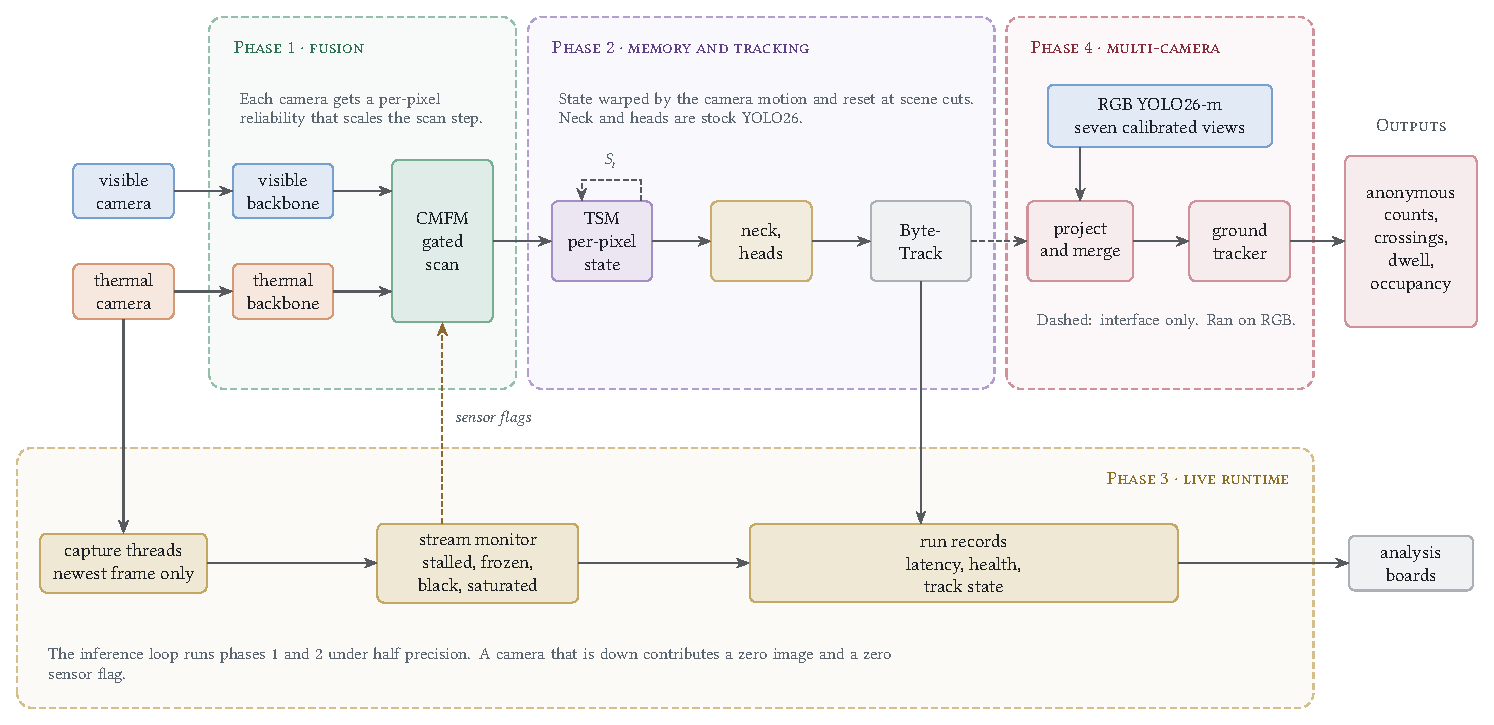
\includegraphics[width=\textwidth]{figures/fig_pipeline.pdf}
\caption{The complete system. Paired visible and thermal cameras pass through the reliability-gated fusion detector, the Temporal State Memory and ByteTrack, inside a live runtime whose stream monitor raises sensor flags. The multi-camera ground-plane layer was run on an RGB-only detector, so its link from the tracker is the interface only.}
\label{fig:pipeline}
\end{figure}

\begin{figure}[!htbp]
\centering
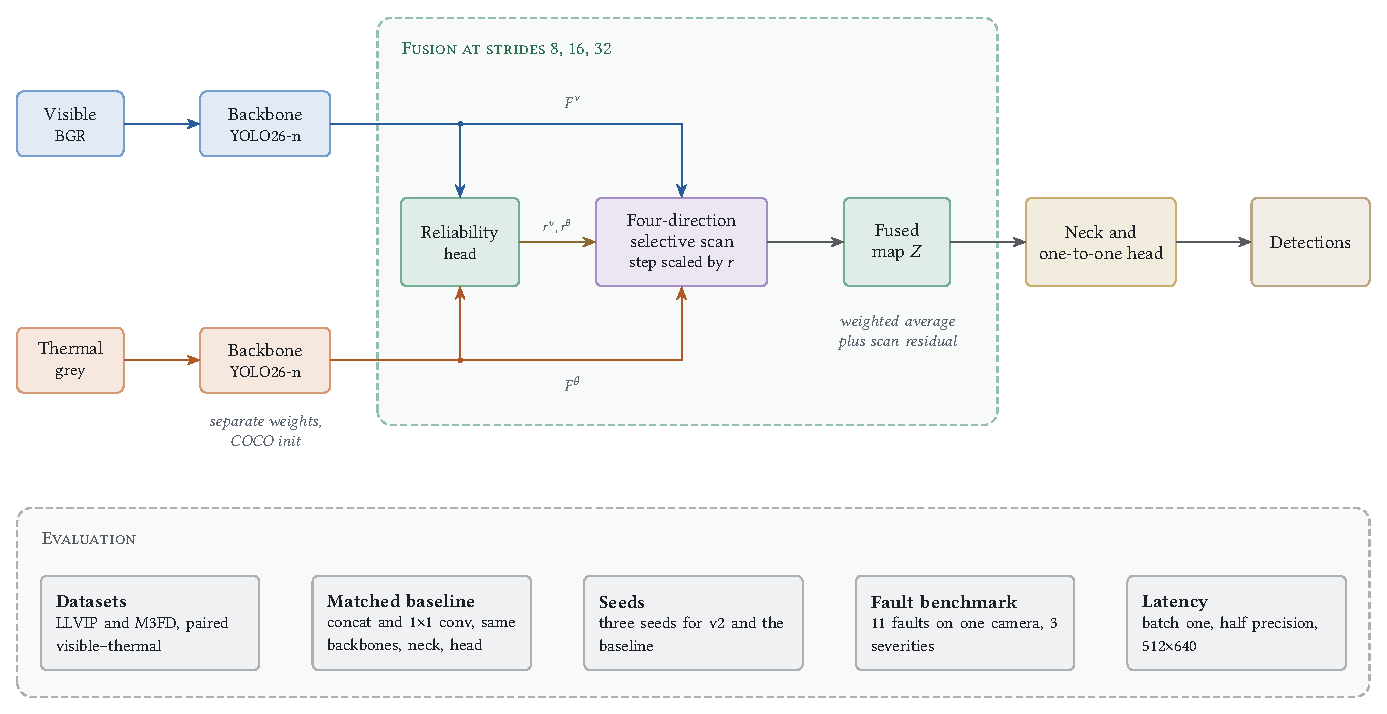
\includegraphics[width=\textwidth]{figures/fig_phase1.pdf}
\caption{The fusion detector on still image pairs. Two YOLO26-n backbones feed a fusion block at strides 8, 16 and 32, in which a reliability head scales the step of a four-direction selective scan. The strip below lists the evaluation of the main paper.}
\label{fig:phaseone}
\end{figure}

\begin{figure}[!htbp]
\centering
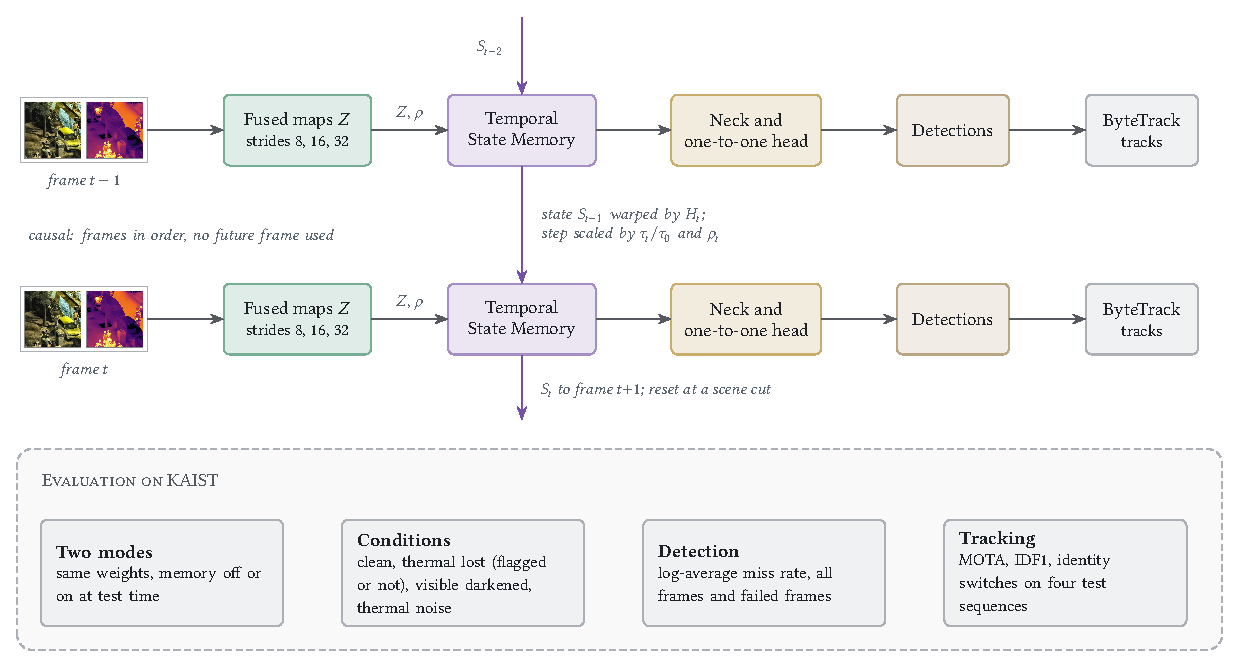
\includegraphics[width=\textwidth]{figures/fig_phase2.pdf}
\caption{Video, the Temporal State Memory and tracking. The fused features of each frame update a per-pixel state carried from frame $t-1$ to frame $t$, warped by the homography and gated by elapsed time and reliability. Detections feed ByteTrack, and KAIST is scored with the memory off and on.}
\label{fig:phasetwo}
\end{figure}

\begin{figure}[!htbp]
\centering
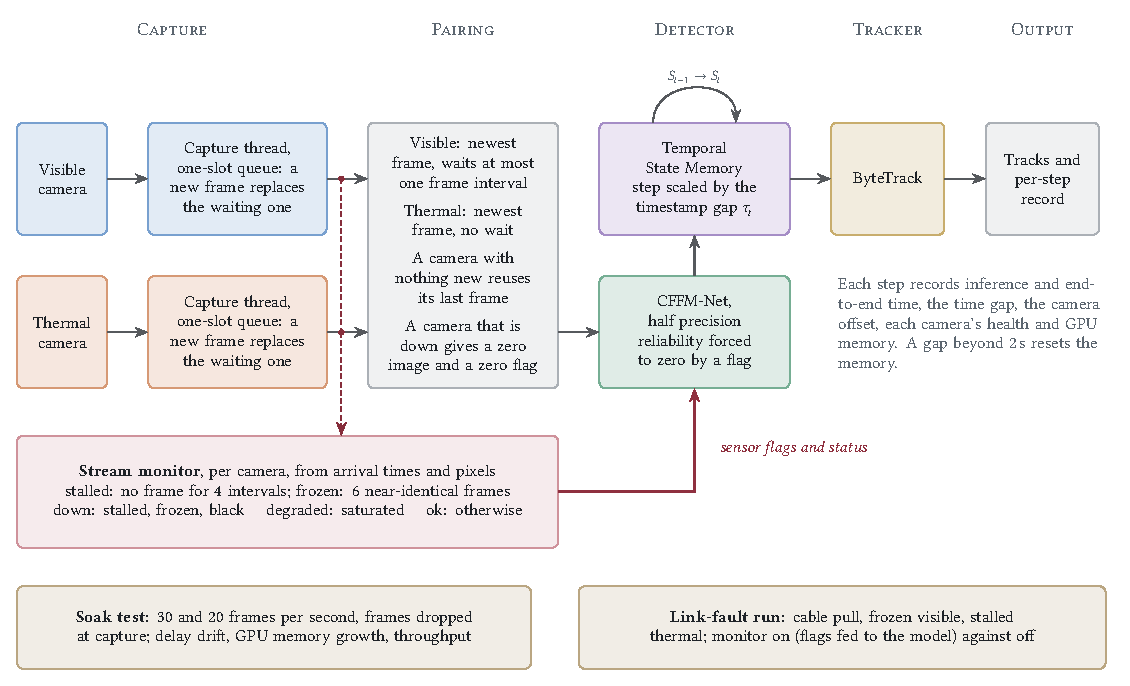
\includegraphics[width=\textwidth]{figures/fig_phase3.pdf}
\caption{The live runtime. Two threaded captures with one-slot queues feed a newest-frame pairing step, then the detector with its memory and ByteTrack. A stream monitor watches each camera and feeds sensor flags back to the detector.}
\label{fig:phasethree}
\end{figure}

\begin{figure}[!htbp]
\centering
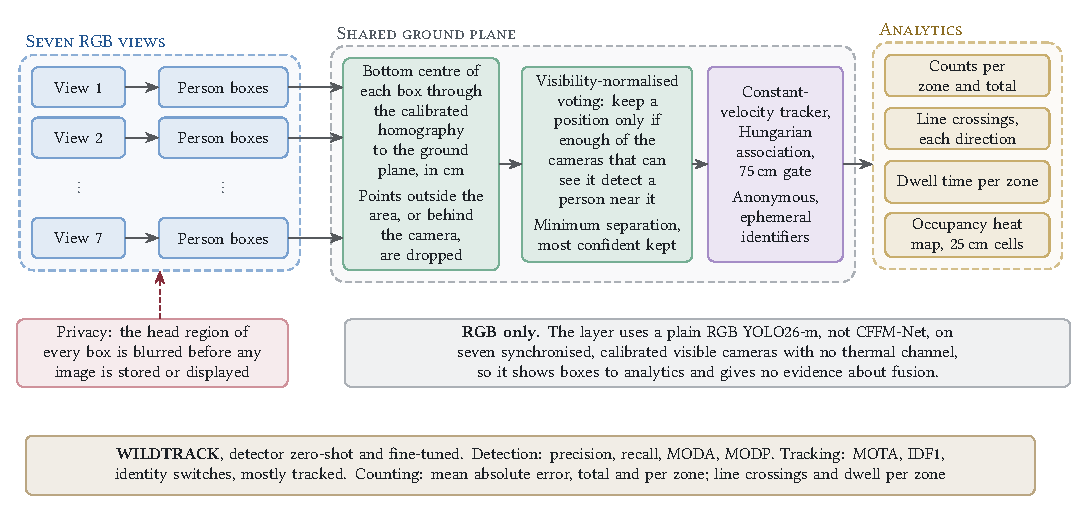
\includegraphics[width=\textwidth]{figures/fig_phase4.pdf}
\caption{The multi-camera layer. Person boxes from each RGB view are projected to a shared ground plane, merged across cameras and tracked anonymously, giving counts, line crossings, dwell time and an occupancy map on WILDTRACK. The layer is RGB-only and gives no evidence about fusion.}
\label{fig:phasefour}
\end{figure}

\begin{figure}[!htbp]
\centering
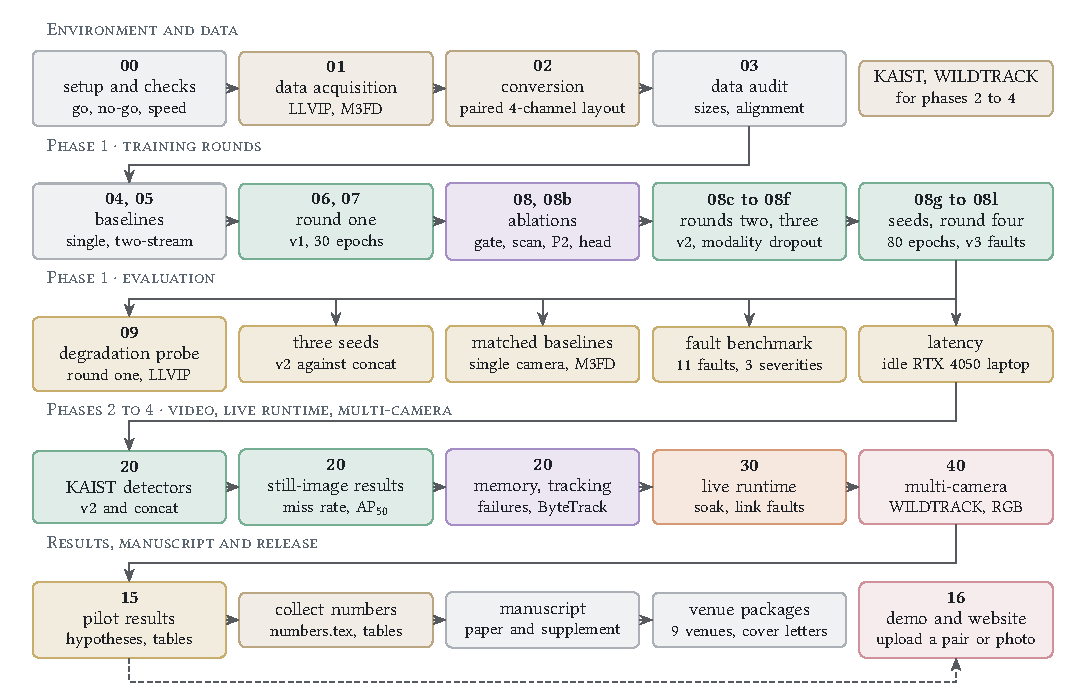
\includegraphics[width=\textwidth]{figures/fig_workflow.pdf}
\caption{The research workflow from data to venue packages: environment and data, the training rounds, the evaluations of each phase, the numbers file that feeds every table, and the manuscript.}
\label{fig:workflow}
\end{figure}

\section{Result figures}
\label{app:resfigs}
Figures~\ref{fig:resmain} to~\ref{fig:resmulticam} plot the measurements behind the tables. Each one is drawn directly from the result files of the repository by a single script, and none of them adds a result that the tables do not hold.

\begin{figure}[!htbp]
\centering
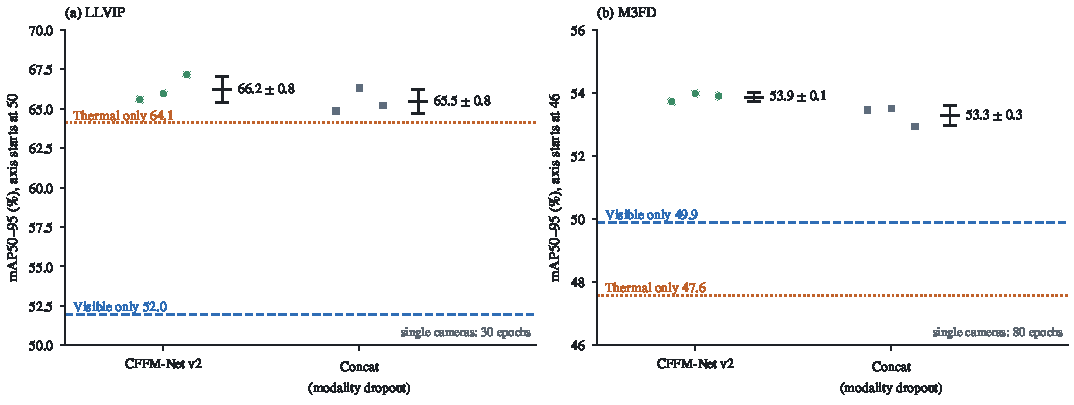
\includegraphics[width=\textwidth]{figures/res_main.pdf}
\caption{mAP$_{50\text{-}95}$ of CFFM-Net v2 and the concatenation baseline with modality dropout on LLVIP and M3FD. Dots are the three seeds and the bars are the mean and sample standard deviation. The dashed and dotted lines are the single-camera YOLO26-n baselines at seed 0, trained for 30 epochs on LLVIP and for a matched 80 epochs on M3FD. The vertical axes do not start at zero.}
\label{fig:resmain}
\end{figure}

\begin{figure}[!htbp]
\centering
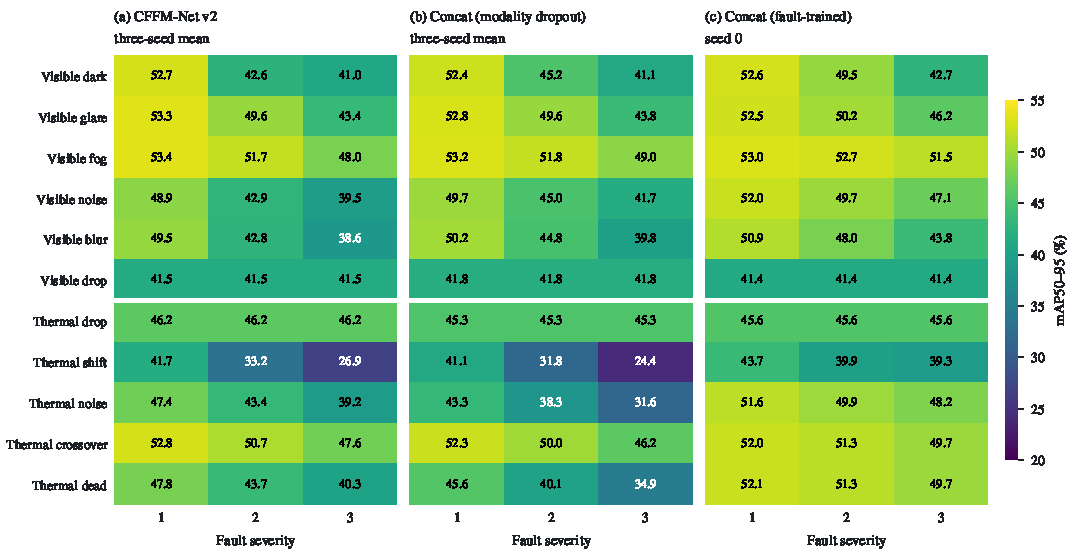
\includegraphics[width=\textwidth]{figures/res_fault_heatmap.pdf}
\caption{M3FD mAP$_{50\text{-}95}$ under eleven sensor faults at three severities. CFFM-Net v2 and the concatenation baseline with modality dropout are means over three seeds, and the fault-trained concatenation baseline is seed 0. Dropping a camera has no severity, so those rows are constant.}
\label{fig:resfaultheat}
\end{figure}

\begin{figure}[!htbp]
\centering
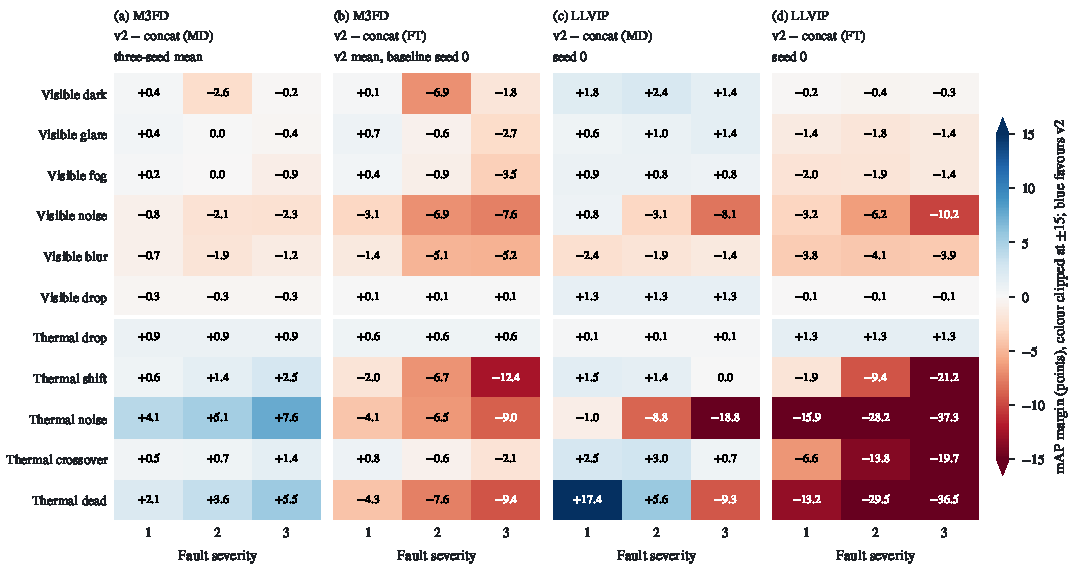
\includegraphics[width=\textwidth]{figures/res_fault_margin.pdf}
\caption{Margin of CFFM-Net v2 over the two concatenation baselines in mAP points, per fault and severity. Blue cells favour v2 and red cells favour the baseline. On M3FD the margin over the modality-dropout baseline is a three-seed mean and the margin over the fault-trained baseline compares the v2 mean with seed 0, and LLVIP is seed 0 throughout. The colour scale is clipped at 15 points, and every cell prints its value.}
\label{fig:resfaultmargin}
\end{figure}

\begin{figure}[!htbp]
\centering
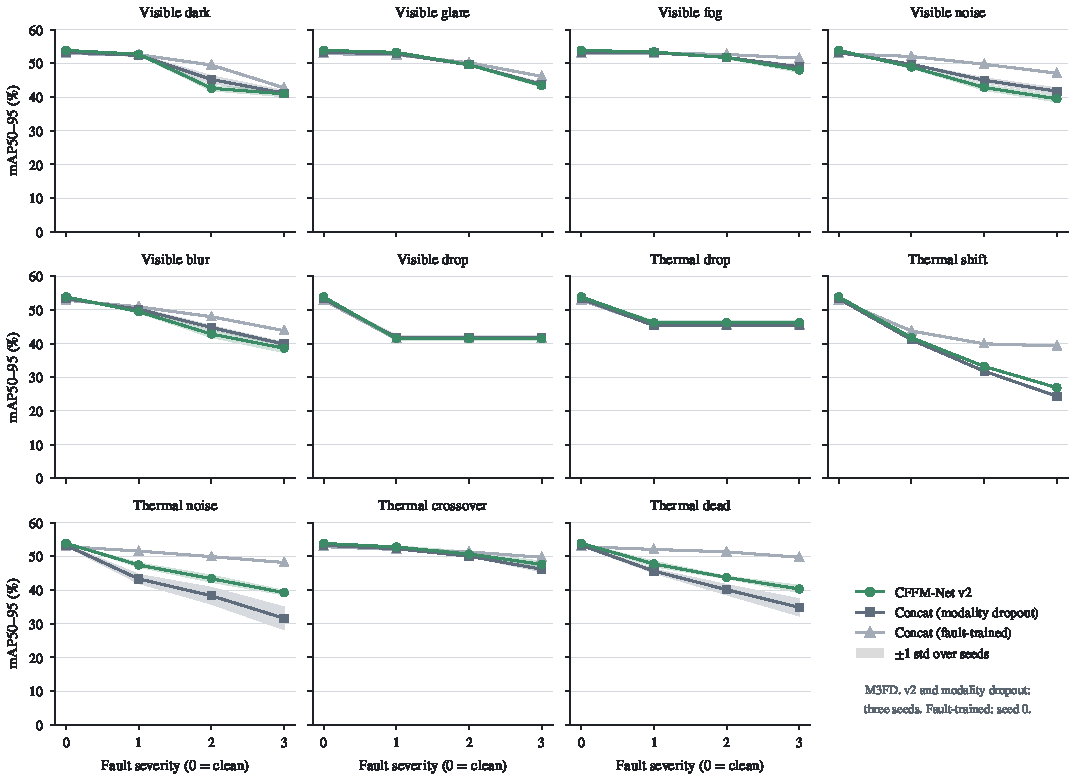
\includegraphics[width=\textwidth]{figures/res_severity_curves.pdf}
\caption{M3FD mAP$_{50\text{-}95}$ against fault severity for each of the eleven faults. Lines for CFFM-Net v2 and the concatenation baseline with modality dropout are three-seed means with a band of one standard deviation, and the fault-trained baseline is seed 0.}
\label{fig:resseverity}
\end{figure}

\begin{figure}[!htbp]
\centering
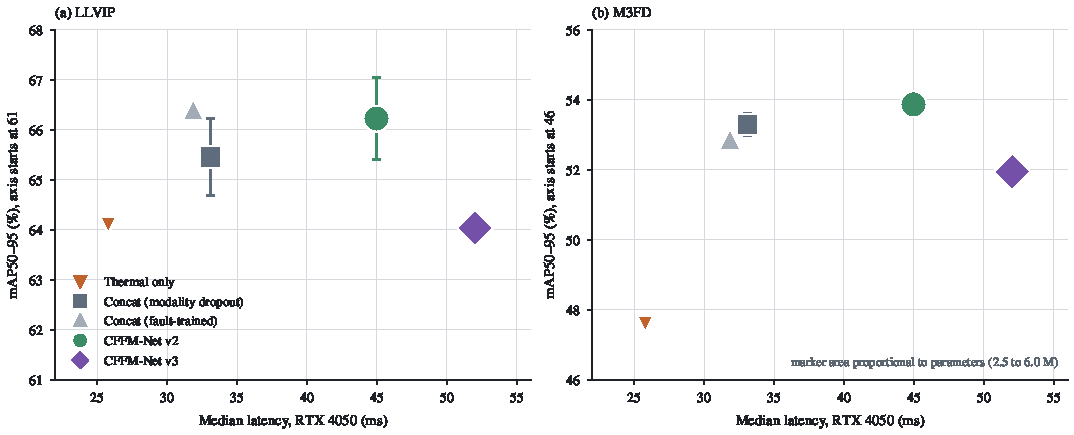
\includegraphics[width=\textwidth]{figures/res_tradeoff.pdf}
\caption{mAP$_{50\text{-}95}$ against median latency on an RTX 4050 Laptop GPU (FP16, batch 1, $640\times512$). Marker area is proportional to the parameter count. CFFM-Net v2 and the modality-dropout baseline are three-seed means with one standard deviation, and the other models are seed 0. The thermal-only model on LLVIP was trained for 30 epochs, and the vertical axes do not start at zero.}
\label{fig:restradeoff}
\end{figure}

\begin{figure}[!htbp]
\centering
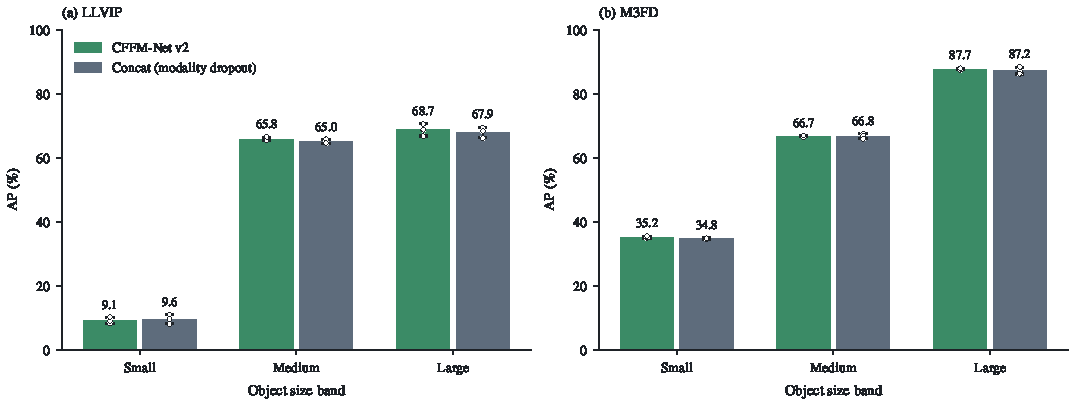
\includegraphics[width=\textwidth]{figures/res_scale.pdf}
\caption{COCO small, medium and large AP of CFFM-Net v2 and the concatenation baseline with modality dropout. Bars are three-seed means with one standard deviation and the dots are the seeds.}
\label{fig:resscale}
\end{figure}

\begin{figure}[!htbp]
\centering
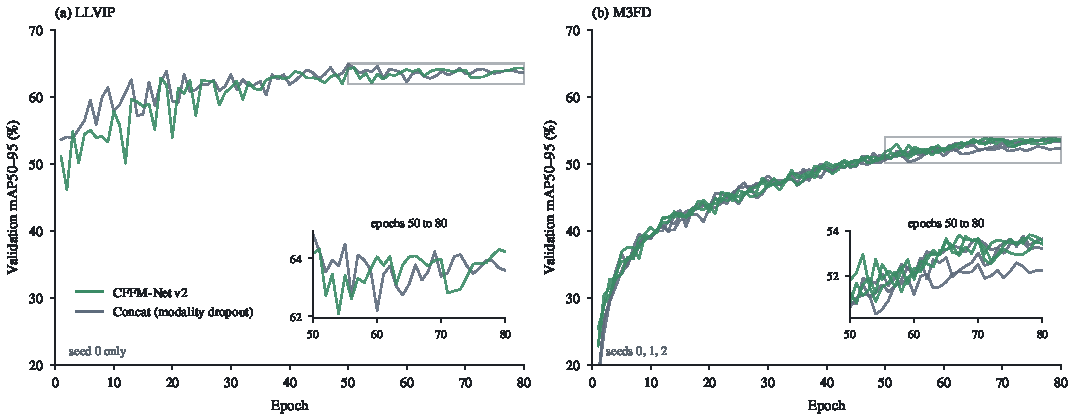
\includegraphics[width=\textwidth]{figures/res_training.pdf}
\caption{Validation mAP$_{50\text{-}95}$ against epoch for CFFM-Net v2 and the concatenation baseline with modality dropout, with epochs 50 to 80 enlarged. LLVIP shows seed 0, the only seed whose training log was kept, and M3FD shows seeds 0 to 2.}
\label{fig:restraining}
\end{figure}

\begin{figure}[!htbp]
\centering
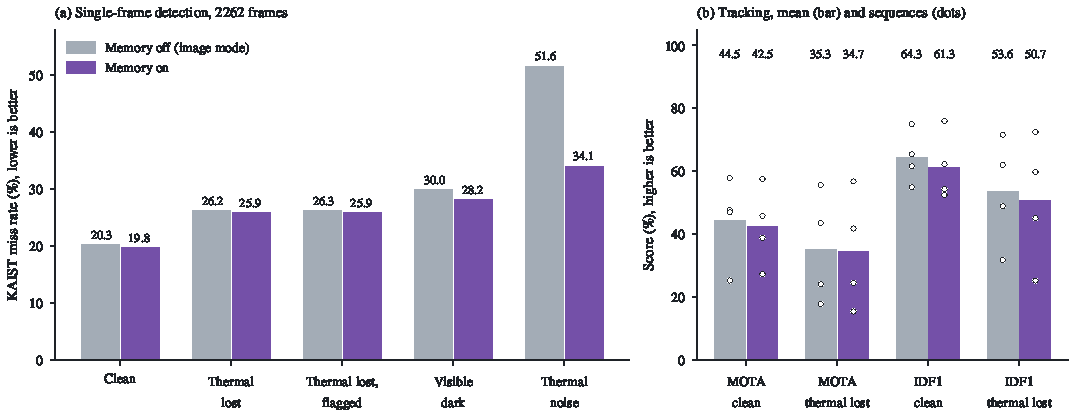
\includegraphics[width=\textwidth]{figures/res_memory.pdf}
\caption{The Temporal State Memory on KAIST. (a) Miss rate over the 2262 validation frames with the memory off and on under each condition, where lower is better. (b) Tracking MOTA and IDF1 as the mean over four sequences, with one dot per sequence.}
\label{fig:resmemory}
\end{figure}

\begin{figure}[!htbp]
\centering
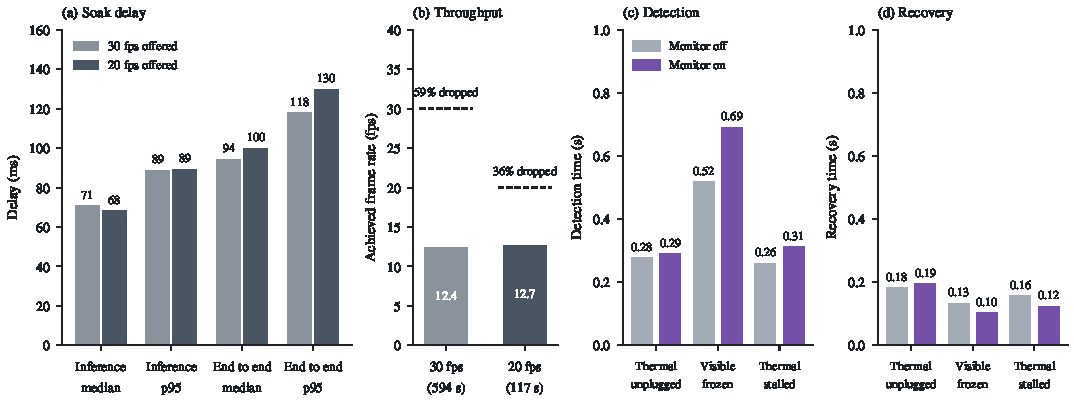
\includegraphics[width=\textwidth]{figures/res_live.pdf}
\caption{The live runtime. (a) Median and 95th-percentile inference and end-to-end delay in the soak runs at 30 and 20 offered frames per second. (b) Achieved frame rate against the offered rate, with the share of frames dropped at capture. (c), (d) Time to detect and to recover from three scripted link faults with the stream monitor off and on, one run each.}
\label{fig:reslive}
\end{figure}

\begin{figure}[!htbp]
\centering
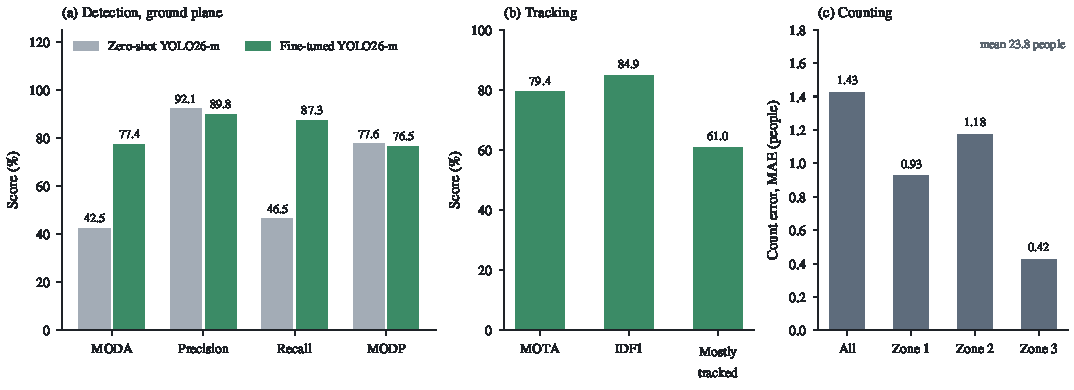
\includegraphics[width=\textwidth]{figures/res_multicam.pdf}
\caption{The multi-camera layer on WILDTRACK with an RGB YOLO26-m detector. (a) Ground-plane detection, zero-shot against fine-tuned. (b) Tracking. (c) Mean absolute count error over the whole ground plane and in three zones.}
\label{fig:resmulticam}
\end{figure}
